\section{Năng lượng liên kết hạt nhân}
\subsection{Tóm tắt lí thuyết}
\begin{tomtat}
	\subsubsection{Hệ thức Einstein về mối liên hệ giữa khối lượng và năng lượng}
	\begin{boxdl}
		Hệ thức mô tả mối liên hệ giữa khối lượng $m$ và năng lượng $E$:
		\begin{equation}
			E=mc^2
		\end{equation}
	\end{boxdl}
	Trong đó:
	\begin{itemize}
		\item $E$: năng lượng toàn phần, đơn vị trong hệ SI là joule $\left(\si{\joule}\right)$;
		\item $m$: khối lượng, đơn vị trong hệ SI là kilogram $\left(\si{\kilogram}\right)$;
		\item $c=\SI{3E8}{\meter/\second}$: tốc độ ánh sáng trong chân không.
	\end{itemize}
\begin{noidung}{}
	Năng lượng trong một phản ứng hạt nhân thường có giá trị nhỏ hơn rất nhiều so với $\SI{1}{\joule}$. Do đó, người ta thường sử dụng đơn vị electron volt
	$$\SI{1}{\electronvolt}=\SI{1.6E-19}{\joule}.$$
\end{noidung}
\begin{note}
	Khối lượng của một vật khi ở trạng thái nghỉ (đứng yên tương đối với người quan sát trong hệ quy chiếu quán tính) được gọi là khối lượng nghỉ, kí hiệu là $m_0$. Năng lượng của vật khi ở trạng thái nghỉ được gọi là năng lượng nghỉ, kí hiệu là $E_0$. Năng lượng toàn phần gồm năng lượng nghỉ và động năng của vật:
	$$E=E_0+W_\text{đ}.$$
\end{note}
	\subsubsection{Khối lượng hạt nhân}
	Do khối lượng hạt nhân nguyên tử lớn hơn rất nhiều so với khối lượng các electron nên khối lượng hạt nhân xấp xỉ bằng khối lượng nguyên tử.\\
	Trong vật lí hạt nhân, khối lượng thường được đo bằng đơn vị khối lượng nguyên tử, kí hiệu là $\si{amu}$ (hoặc $\si{u}$); $\SI{1}{amu}$ có giá trị bằng $\dfrac{1}{12}$ khối lượng của một nguyên tử của đồng vị $\ce{^{12}_6C}$:
	\begin{equation}
		\SI{1}{amu}=\dfrac{1}{12}\cdot\xsi{\dfrac{12}{6,02214\cdot10^{23}}}{\gram}\approx\SI{1.66054E-27}{\kilogram}=\SI{931.5}{\mega\electronvolt/c^2}
	\end{equation}
	\subsubsection{Năng lượng liên kết hạt nhân}
	\paragraph{Lực hạt nhân}
	\begin{dn}
		Lực hạt nhân 
		\begin{itemize}
			\item là lực tương tác giữa các nucleon và có tác dụng liên kết các nucleon với nhau để tạo thành hạt nhân;
			\item  có bản chất liên quan tới tương tác mạnh, có cường độ rất lớn so với lực điện từ và lực hấp dẫn;
			\item  chỉ tác dụng trong phạm vi kích thước hạt nhân (khoảng $\SI{E-15}{\meter}$);
			\item  không phụ thuộc vào điện tích và khối lượng các nucleon.
		\end{itemize}
	\end{dn}
	\paragraph{Độ hụt khối}
\begin{dn}
		Độ hụt khối  của hạt nhân bằng hiệu giữa tổng khối lượng của các nucleon riêng rẽ tạo thành hạt nhân $\ce{^A_Z X}$ và khối lượng của hạt nhân $\ce{^A_Z X}$:
	\begin{equation}
		\Delta m=\left[Zm_p+\left(A-Z\right)m_n\right]-m_X.
	\end{equation}
\end{dn}
	\subsubsection{Năng lượng liên kết}
	\begin{dn}
		Năng lượng liên kết hạt nhân bằng năng lượng tối thiểu để tách một hạt nhân thành các nucleon riêng rẽ hoặc bằng năng lượng toả ra khi các nucleon riêng rẽ kết hợp thành hạt nhân
		\begin{equation}
			E_\text{lk}=\Delta mc^2.
		\end{equation}
		Năng lượng liên kết hạt nhân thường được đo bằng đơn vị $\si{\mega\electronvolt}$.
	\end{dn}
	\subsubsection{Năng lượng liên kết riêng hạt nhân}
	\begin{dn}
		Năng lượng liên kết riêng hạt nhân là năng lượng liên kết tính cho một nucleon
		\begin{equation}
			E_\text{lkr}=\dfrac{E_\text{lk}}{A}.
		\end{equation}
	\end{dn}
	\begin{note}
		Hạt nhân có năng lượng liên kết riêng càng lớn thì càng bền vững.\\ 
		Những hạt nhân có số khối $50<A<80$ là các hạt nhân bền. Các hạt nhân bền có năng lượng liên kết riêng lớn nhất vào cỡ $\SI{8.8}{\mega\electronvolt/nucleon}$.
	\end{note}
\end{tomtat}
\subsection{Ví dụ minh hoạ}
\begin{dang}{Vận dụng hệ thức Einstein về mối liên hệ giữa khối lượng và năng lượng}
\end{dang}
		\begin{vd}
			Do sự phát bức xạ nên mỗi ngày $\left(\SI{86400}{\second}\right)$ khối lượng Mặt Trời giảm một lượng $\SI{3.744E14}{\kilogram}$. Biết tốc độ ánh sáng trong chân không là $\SI{3E8}{\meter/\second}$. Công suất bức xạ trung bình của Mặt Trời bằng bao nhiêu?
			\loigiai{
			Công suất bức xạ trung bình của Mặt Trời:
			$$\calP=\dfrac{E}{t}=\dfrac{mc^2}{t}=\dfrac{\left(\SI{3.744E14}{\kilogram}\right)\cdot\left(\SI{3E8}{\meter/\second}\right)^2}{\SI{86400}{\second}}=\SI{3.9e20}{\mega\watt}.$$
			}
		\end{vd}
	% ===========================================================
	\begin{vd}
	Công suất bức xạ toàn phần của Mặt Trời là $\calP=\SI{3.9E26}{\watt}$. Phản ứng hạt nhân trong lòng Mặt Trời là phản ứng tổng hợp hydrogen thành helium  và lượng helium tạo thành trong một năm (365 ngày) là $\SI{1.945E19}{\kilogram}$. Tính khối lượng hydrogen tiêu thụ một năm trên Mặt Trời.
	\loigiai{
	Năng lượng Mặt Trời tiêu thụ trong 1 năm:
	$$E=\calP t=\left(\SI{3.9E26}{\watt}\right)\cdot365\cdot24\cdot\left(\SI{3600}{\second}\right)	=\SI{1.23E34}{\joule}.$$
	Phần khối lượng Mặt Trơi bị giảm đi mỗi năm:
	$$\Delta m=\dfrac{E}{c^2}=\dfrac{\SI{1.23E34}{\joule}}{\left(\SI{3E8}{\meter/\second}\right)^2}=\SI{1.3667E17}{\kilogram}.$$
	Lượng hydrogen tiêu hao hằng năm:
	$$m_{\ce{H}}=m_{\ce{He}}+\Delta m=\SI{1.3667E17}{\kilogram}+\SI{1.945E19}{\kilogram}\approx\SI{1.958E19}{\kilogram}.$$
	}
	\end{vd}
\begin{dang}{Xác định được độ hụt khối, năng lượng liên kết và năng lượng liên kết riêng của hạt nhân}
	\end{dang}
\begin{vd}
Các hạt nhân deuterium $\ce{^2_1D}$; tritium $\ce{^3_1T}$; helium $\ce{^4_2He}$ có năng lượng liên kết lần lượt là $\SI{2.22}{\mega\electronvolt}$; $\SI{8.49}{\mega\electronvolt}$ và $\SI{28.16}{\mega\electronvolt}$. Hãy sắp xếp các hạt nhân trên theo thứ tự giảm dần độ bền vững.
\loigiai{
\begin{itemize}
	\item Năng lượng liên kết riêng của $\ce{^2_1D}$:
	$$W_\text{lkrD}=\dfrac{W_\text{lkD}}{A_\text{D}}=\dfrac{\SI{2.22}{\mega\electronvolt}}{2}=\SI{1.11}{\mega\electronvolt/nucleon}.$$
	\item Năng lượng liên kết riêng của $\ce{^3_1T}$:
	$$W_\text{lkrT}=\dfrac{W_\text{lkT}}{A_\text{T}}=\dfrac{\SI{8.49}{\mega\electronvolt}}{3}=\SI{2.83}{\mega\electronvolt/nucleon}.$$
	\item Năng lượng liên kết riêng của $\ce{^4_2He}$:
	$$W_\text{lkrHe}=\dfrac{W_\text{lkHe}}{A_\text{He}}=\dfrac{\SI{28.16}{\mega\electronvolt}}{4}=\SI{7.04}{\mega\electronvolt/nucleon}.$$
\end{itemize}	
Vậy sắp xếp theo thứ tự giảm dần độ bền vững là: $\ce{^4_2He}$; $\ce{^3_1T}$; $\ce{^2_1D}$.
}
\end{vd}
% ===================================================================
\begin{vd}
Đồng vị của cobalt $\left(\ce{^{60}_{27}Co}\right)$ có khối lượng hạt nhân là $m_{\ce{Co}}=\SI{59.934}{u}$. Khối lượng của các hạt proton; neutron lần lượt là $m_p=\SI{1.0073}{u}$; $m_n=\SI{1.0087}{u}$ và $\SI{1}{u}=\SI{931.5}{\mega\electronvolt/c^2}$. Tính:
\begin{enumerate}[label=\alph*)]
	\item độ hụt khối của hạt nhân cobalt;
	\item năng lượng liên kết và năng lượng liên kết riêng của hạt nhân cobalt.
\end{enumerate}
\loigiai{
\begin{enumerate}[label=\alph*)]
	\item Độ hụt khối của hạt nhân cobalt:
	$$\Delta m=27m_p+\left(60-27\right)m_n-m_{\ce{Co}}=\SI{0.5502}{u}.$$
	\item \begin{itemize}
		\item Năng lượng liên kết của hạt nhân cobalt:
		$$W_\text{lk}=\Delta mc^2=\SI{0.5502}{uc^2}=0,5502\cdot\SI{931.5}{\mega\electronvolt}=\SI{512.5113}{\mega\electronvolt}.$$
		\item Năng lượng liên kết riêng của hạt nhân cobalt:
		$$W_\text{lkr}=\dfrac{W_\text{lk}}{A}=\dfrac{\SI{512.5113}{\mega\electronvolt}}{60}=\SI{8.5418}{\mega\electronvolt/\text{nucleon}}.$$
	\end{itemize}
	
\end{enumerate}	
}
\end{vd}
% =============================================
\begin{vd}
	Cho khối lượng hạt nhân $\ce{^{24}_{12} Mg}$, khối lượng proton và khối lượng neutron lần lượt là $\SI{23.97846}{u}$; $\SI{1.0073}{u}$ và $\SI{1.0087}{u}$. Biết $\SI{1}{u}=\SI{1.66055e-27}{\kilogram}=\SI{931.5}{\mega\electronvolt/c^2}$. Tính năng lượng cần thiết để tách các hạt nhân $\ce{^{24}_{12} Mg}$ có trong $\SI{1}{\gram}$ magie thành các nucleon riêng lẻ.
	\loigiai{
	Số hạt nhân $\ce{^{24}_{12} Mg}$ có trong $m=\SI{1}{\gram}$ magie:
	$$N_{\ce{Mg}}=\dfrac{m}{m_{\ce{Mg}}}=\dfrac{\SI{E-3}{\kilogram}}{23,97846\cdot\left(\SI{1.66055E-27}{\kilogram}\right)}=\SI{2.51E22}{\text{hạt}}.$$
	Năng lượng liên kết của $\ce{^{24}_{12} Mg}$:
	$$W_\text{lk}=\left(12m_p+12m_n-m_{\ce{Mg}}\right)c^2=\SI{198.91}{\mega\electronvolt}.$$
	Năng lượng cần thiết để tách các hạt nhân $\ce{^{24}_{12} Mg}$ trong $\SI{1}{\gram}$ là
	$$E=N_{\ce{Mg}}W_\text{lk}=\SI{5E24}{\mega\electronvolt}.$$
	}
\end{vd}
\subsection{Bài tập}
\subsubsection{Trắc nghiệm nhiều phương án lựa chọn}
\setcounter{ex}{0}
\Opensolutionfile{ans}[ans/VN12-Y24-PH-SYL-026P-TN]
% ===================================================================
\begin{ex}
	Chọn cụm từ phù hợp để hoàn thành nhận định sau: \\
	"Khối lượng của một hạt nhân bất kì \dots tổng khối lượng của các nucleon riêng lẽ cấu tạo thành hạt nhân đó".
	\choice
	{luôn lớn hơn}
	{\True luôn nhỏ hơn}
	{luôn bằng}
	{có lúc lớn hơn, có lúc nhỏ hơn}
	\loigiai{}
\end{ex}
% ===================================================================
\begin{ex}
	Một hạt nhân có độ hụt khối càng lớn thì hạt nhân đó
	\choice
	{\True có năng lượng liên kết càng lớn}
	{có năng lượng liên kết không đổi}
	{có năng lượng liên kết càng nhỏ}
	{càng bền vững}
	\loigiai{}
\end{ex}
% ===================================================================
\begin{ex}
	Năng lượng liên kết của hạt nhân bằng
	\choice
	{năng lượng trung bình liên kết mỗi nucleon trong hạt nhân}
	{năng lượng cần thiết để tách một nucleon khỏi hạt nhân}
	{\True năng lượng cần thiết để tách rời tất cả các nucleon trong hạt nhân}
	{tích của khối lượng hạt nhân với bình phương của tốc độ ánh sáng trong chân không}
	\loigiai{}
\end{ex}
% ===================================================================
\begin{ex}
	Năng lượng liên kết riêng của hạt nhân có giá trị	
	\choice
	{lớn nhất đối với các hạt nhân nhẹ}
	{lớn nhất đối với các hạt nhân nặng}
	{\True lớn nhất đối với các hạt nhân trung bình}
	{như nhau với mọi hạt nhân}
	\loigiai{}
\end{ex}
% ===================================================================
\begin{ex}
	Độ hụt khối của một hạt nhân $\ce{_Z^AX}$
	\choice
	{là đại lượng đặc trưng cho mức độ bền vững của hạt nhân}
	{\True được xác định bằng biểu thức $\Delta m=\left[Z m_{p}+\left(A-Z\right) m_{n}\right]-m_{x}$}
	{càng lớn khi số khối của hạt nhân càng lớn}
	{là đại lượng đặc trưng cho mức độ phổ biến của hạt nhân}
	\loigiai{}
\end{ex}
% ===================================================================
\begin{ex}
	Chỉ ra phát biểu \textbf{sai}.
	\choice
	{Hệ thức Einstein về mối liên hệ giữa năng lượng và khối lượng là $E=m c^2$}
	{Khối lượng nghỉ là khối lượng của một vật khi ở trạng thái nghỉ}
	{Khối lượng của một nguyên tử có giá trị gần bằng khối lượng của hạt nhân nguyên tử đó}
	{\True Một hạt nhân có số khối $A$ thì khối lượng của nó luôn lớn hơn $\xsi{A}{\left(anu\right)}$}
	\loigiai{}
\end{ex}
% ===================================================================
\begin{ex}
	Năng lượng liên kết riêng của hạt nhân
	\choice
	{\True càng lớn thì hạt nhân càng bền vững}
	{có thể bằng 0 đối với các hạt nhân đặc biệt}
	{càng nhỏ thì hạt nhân càng bền vững}
	{có thể dương hoặc âm}
	\loigiai{}
\end{ex}
% ===================================================================
\begin{ex}
	Đồ thị nào dưới đây mô tả \textbf{gần đúng} mối liên hệ giữa năng lượng liên kết riêng $\left(E_{\text{lkr}}\right)$ với số nucleon $\left(A\right)$?
	\choice
	{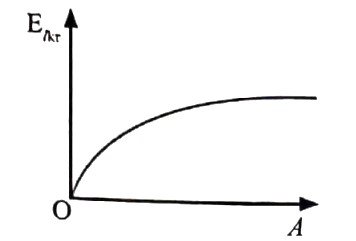
\includegraphics[width=0.42\linewidth]{figs/VN12-Y24-PH-SYL-027P-2a}}
	{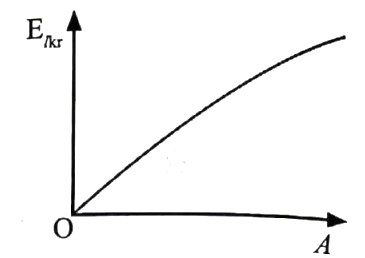
\includegraphics[width=0.42\linewidth]{figs/VN12-Y24-PH-SYL-027P-2b}}
	{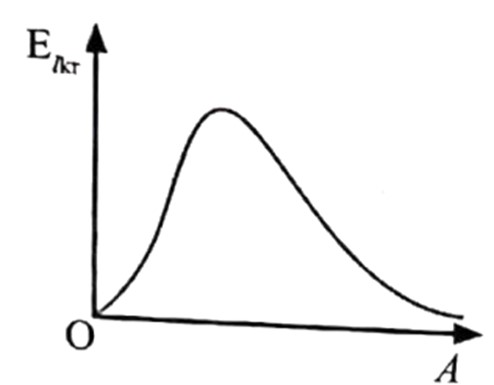
\includegraphics[width=0.42\linewidth]{figs/VN12-Y24-PH-SYL-027P-2c}}
	{\True 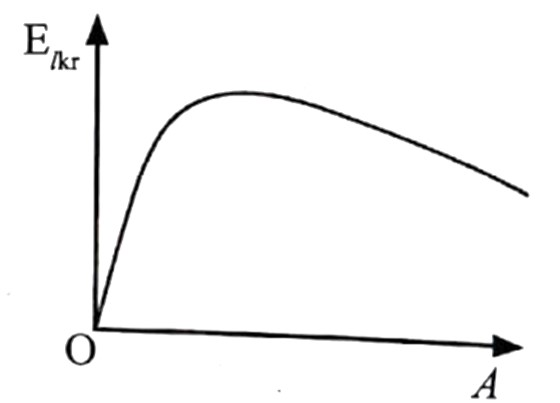
\includegraphics[width=0.42\linewidth]{figs/VN12-Y24-PH-SYL-027P-2d}}
	\loigiai{}
\end{ex}
% ===================================================================
\begin{ex}
	Nhận định nào sau đây \textbf{sai} khi nói về lực hạt nhân?
	\choice
	{\True Lực hạt nhân có bản chất là lực hấp dẫn vì nó giúp kết nối các nucleon lại với nhau}
	{Lực hạt nhân có bản chất là lực tương tác mạnh}
	{Lực hạt nhân có cường độ lớn hơn nhiều lần so với cường độ của lực tĩnh điện}
	{Lực hạt nhân có phạm vi tác dụng trong bán kính hạt nhân}
	\loigiai{}
\end{ex}
% ===================================================================
\begin{ex}
	Chọn đáp án \textbf{đúng}.\\
	Dựa vào đồ thị biểu diễn năng lượng liên kết riêng của các hạt nhân theo số khối, sự sắp xếp theo độ bền vững tăng dần của 3 hạt nhân vàng $\left(\ce{Au}\right)$, chlorine $\left(\ce{Cl}\right)$ và sắt $\left(\ce{Fe}\right)$ là
	\begin{center}
		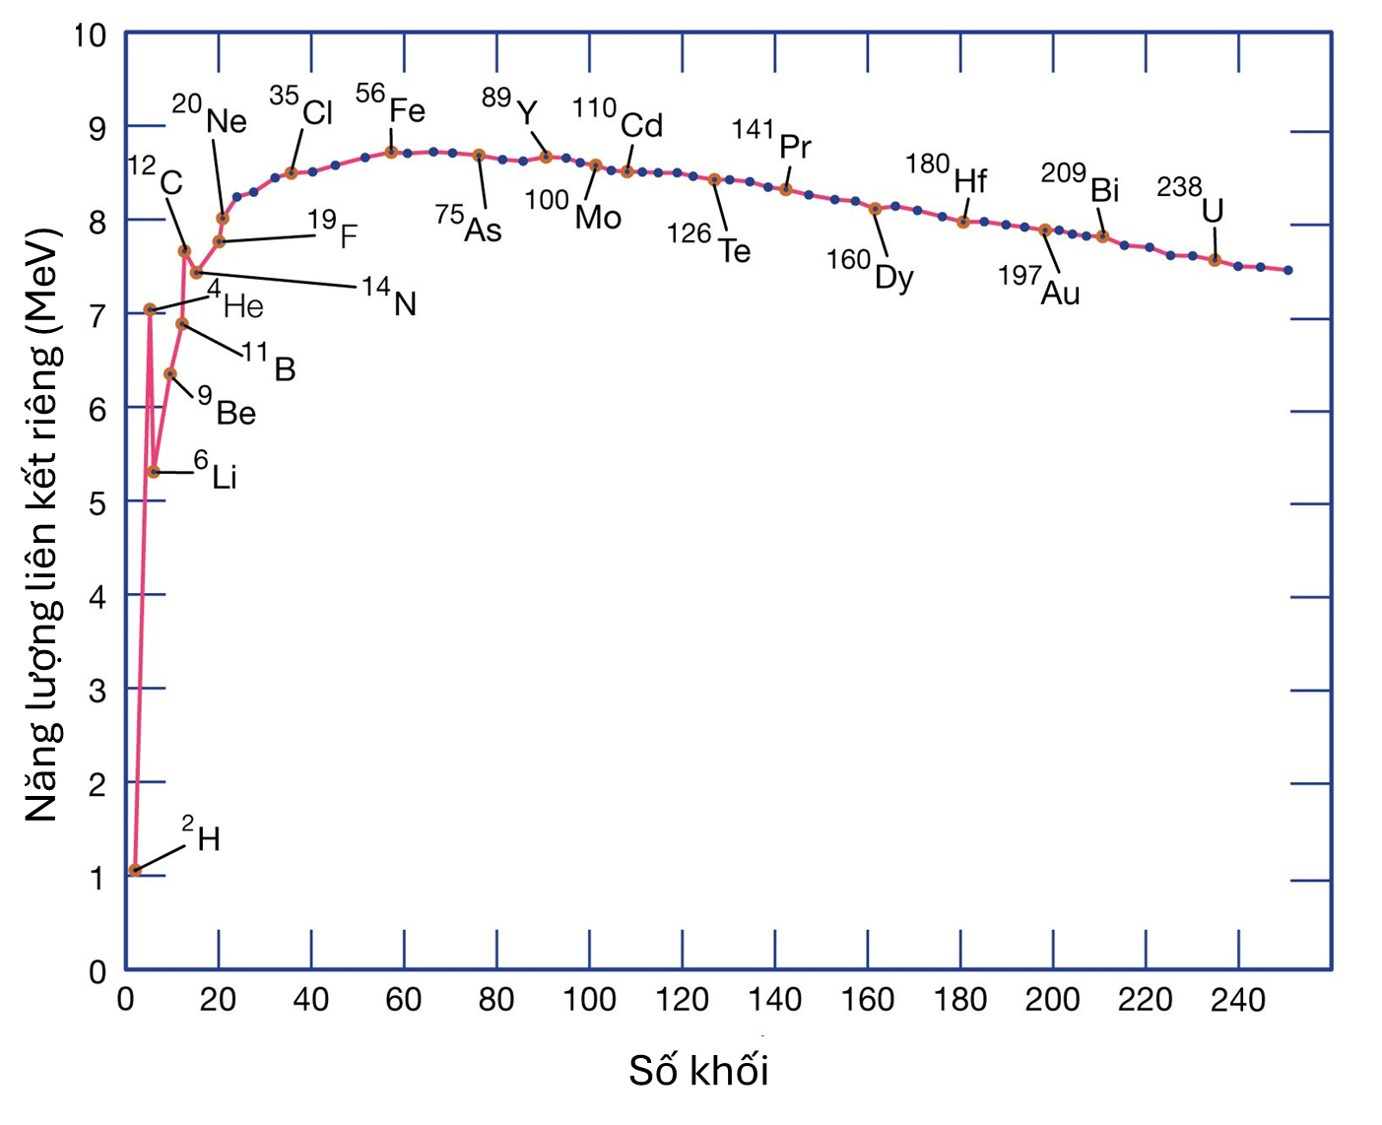
\includegraphics[width=0.7\linewidth]{figs/VN12-Y24-PH-SYL-027P-3}
	\end{center}
	\choice
	{$\ce{Cl}$, $\ce{Au}$, $\ce{Fe}$}
	{$\ce{Fe}$, $\ce{Au}$, $\ce{Cl}$, }
	{\True $\ce{Au}$, $\ce{Cl}$, $\ce{Fe}$}
	{$\ce{Cl}$, $\ce{Fe}$, $\ce{Au}$}
	\loigiai{}
\end{ex}
% ===================================================================
\begin{ex}
	Hạt $\alpha$ có độ hụt khối $\SI{0.0308}{amu}$. Năng lượng liên kết của hạt này bằng	
	\choice
	{$\SI{23.52}{\mega\electronvolt}$}
	{$\SI{25.72}{\mega\electronvolt}$}
	{$\SI{24.72}{\mega\electronvolt}$}
	{\True $\SI{28.70}{\mega\electronvolt}$}
	\loigiai{
		$E_{\text{lk}}=\Delta m\cdot c^2=0,0308\cdot931,5\approx\SI{28.70}{\mega\electronvolt}.$
	}
\end{ex}
% ===================================================================
\begin{ex}
	Nếu năng lượng liên kết của hạt nhân helium $\ce{_2^4He}$ là $\SI{28.8}{\mega\electronvolt}$ thì năng lượng liên kết riêng của nó là
	\choice
	{\True $\SI{7.20}{\mega\electronvolt/nucleon}$}
	{$\SI{14.1}{\mega\electronvolt/nucleon}$}
	{$\SI{0.72}{\mega\electronvolt/nucleon}$}
	{$\SI{1.4}{\mega\electronvolt/nucleon}$}
	\loigiai{
		Năng lượng liên kết riêng của $\ce{^4_2He}$: $E_{\text{lkr}}=\dfrac{E_{\text{lk}}}{A}=\dfrac{28,8}{4}=\SI{7.20}{\mega\electronvolt/nucleon}$.
	}
\end{ex}
% ===================================================================
\begin{ex}
	Các hạt nhân $\ce{_6^{12}C}$, $\ce{_8^{16}O}$, ${ }_2^4 \mathrm{He}$ có năng lượng liên kết lần lượt là $92,16 \mathrm{MeV} ; 127,6 \mathrm{MeV} ; 28,3 \mathrm{MeV}$. Thứ tự giảm dần về mức độ bền vững của hạt nhân là	
	\choice
	{$\ce{_2^4He}$, $\ce{_8^{16}O}$, $\ce{_6^{12}C}$}
	{\True $\ce{_8^{16}O}$, $\ce{_6^{12}C}$, $\ce{_2^4He}$}
	{$\ce{_6^{12}C}$, $\ce{_2^4He}$, $\ce{_8^{16}O}$}
	{$\ce{_2^4He}$, $\ce{_6^{12}C}$, $\ce{_8^{16}O}$}
	\loigiai{}
\end{ex}
% ===================================================================
\begin{ex}
	Một hạt nhân có 8 proton và 9 neutron. Năng lượng liên kết riêng của hạt nhân này bằng $\SI{7.75}{\mega\electronvolt/nucleon}$. Biết $m_p=\SI{1.0073}{amu}$, $ m_n=\SI{1.0087}{amu}$. Khối lượng của hạt nhân đó bằng bao nhiêu amu?
	\choice
	{$\SI{16.545}{amu}$}
	{$\SI{17.138}{amu}$}
	{\True $\SI{16.995}{amu}$}
	{$\SI{17.243}{amu}$}
	\loigiai{
		$E_{\text{lk}}=\left(8+9\right)\cdot\SI{7.75}{\mega\electronvolt}$; $\Delta m=\dfrac{E_{\text{lk}}}{931,5}$\\
		$m_X=\left(8m_p+9m_n\right)-\Delta m=\SI{16.995}{amu}$.
	}
\end{ex}
% ===================================================================
\begin{ex}
	Cho khối lượng nguyên tử helium là $m_{\ce{He}}=\SI{4.003}{amu}$; khối lượng electron là $m_e=\SI{0.000549}{amu}$. Khối lượng của hạt $\alpha$ là	
	\choice
	{\True $\SI{4.001902}{amu}$}
	{$\SI{4.000921}{amu}$}
	{$\SI{4.000975}{amu}$}
	{$\SI{4.002654}{amu}$}
	\loigiai{
		$m_{\alpha}=m_{\ce{He}}-2m_e=\SI{4.001902}{amu}$.
	}
\end{ex}
% ===================================================================
\begin{ex}
	Cho khối lượng các nguyên tử oxygen và hydrogen lần lượt là $\SI{15.999}{amu}$; $\SI{1.0078}{amu}$. Số nguyên tử oxygen có trong $\SI{5}{\gram}$ nước xấp xỉ bằng
	\choice
	{\True $\SI{1.67E23}{}$}
	{$\SI{1.51E23}{}$}
	{$\SI{6.02E23}{}$}
	{$\SI{3.34E23}{}$}
	\loigiai{}
\end{ex}
% ===================================================================
\begin{ex}
	Cho các hạt nhân sau $\ce{_{92}^{238}U}$, $\ce{_{92}^{235}U}$, $\ce{_{11}^{23}Na}$, $\ce{_{79}^{197}Au}$. Sắp xếp các hạt nhân nói trên theo mức độ bền vững tăng dần, biết rằng khối lượng của các hạt nhân nói trên và khối lượng của proton, neutron lần lượt là $m_{\ce{U^{238}}}=\SI{238.050788}{amu}$; $m_{\ce{U^{235}}}=\SI{234.993422}{amu}$, $m_{\ce{Na^{23}}}=\SI{22.983730}{amu}$, $m_{\ce{Au^{197}}}=\SI{196.966552}{amu}$, $m_{p}=\SI{1.007276}{amu}$ và $m_{n}=\SI{1.008665}{amu}$.
	\choice
	{$\ce{_{11}^{23}Na}$, $\ce{_{79}^{197}Au}$, $\ce{_{92}^{235}U}$, $\ce{_{92}^{238}U}$}
	{$\ce{_{92}^{238}U}$, $\ce{_{92}^{235}U}$, $\ce{_{11}^{23}Na}$, $\ce{_{79}^{197}Au}$}
	{\True $\ce{_{92}^{238}U}$, $\ce{_{92}^{235}U}$, $\ce{_{79}^{197}Au}$, $\ce{_{11}^{23}Na}$}
	{$\ce{_{11}^{23}Na}$, $\ce{_{79}^{197}Au}$, $\ce{_{92}^{238}U}$, $\ce{_{92}^{235}U}$}
	\loigiai{
		Năng lượng liên kết riêng của các hạt nhân nói trên lần lượt là:
		$E_{\text{lkr}\left(U238\right)}\approx\SI{7.37}{\mega\electronvolt/\text{nucleon}}, E_{\text{lkr}\left(U235\right)}\approx\SI{7.59}{\mega\electronvolt/\text{nucleon}}, E_{\text{lkr}\left(Na23\right)}\approx\SI{8.11}{\mega\electronvolt/\text{nucleon}}, E_{\text{lkr}\left(Au197\right)}\approx\SI{7.71}{\mega\electronvolt/\text{nucleon}}$.\\
		Thứ tự tăng dần về mức độ bền vững hạt nhân là: $\ce{_{92}^{238}U}$, $\ce{_{92}^{235}U}$, $\ce{_{79}^{197}Au}$, $\ce{_{11}^{23}Na}$
	}
\end{ex}
% ===================================================================
\begin{ex}
	Cho khối lượng của proton, neutron, hạt nhân $\ce{_1^3T}$, hạt nhân $\ce{_{95}^{244}Am}$ lần lượt là $m_{p}=\SI{1.007276}{amu}$,  $m_{n}=\SI{1.008665}{amu}$, $m_{T}=\SI{3.016049}{amu}$ và $m_{\ce{Am}}=\SI{244.064279}{amu}$. Nhận xét nào sau đây \textbf{đúng}?
	\choice
	{Hai hạt nhân này có độ hụt khối bằng nhau}
	{\True Năng lượng liên kết của $\ce{_{95}^{244}Am}$ lớn hơn năng lượng liên kết của $\ce{_1^3T}$}
	{Năng lượng liên kết riêng của ${ }_{95}^{244} \mathrm{Am}$ nhỏ hơn năng lượng liên kết riêng của ${ }_1^3 \mathrm{~T}$}
	{Mức độ bền vững của hai hạt nhân ${ }_1^3 \mathrm{~T}$ và ${ }_{95}^{244} \mathrm{Am}$ là bằng nhau}
	\loigiai{}
\end{ex}
% ===================================================================
\begin{ex}
	Cho ba hạt nhân X, Y và Z có số nucleon tương ứng là $A_X$, $A_Y$ và $A_Z$ với $A_X=2 A_Y=0,5 A_Z$. Biết năng lượng liên kết riêng của từng hạt nhân tương ứng là $\Delta E_X$, $\Delta E_Y$ và $\Delta E_Z$ với $\Delta E_Z<\Delta E_X<\Delta E_Y$. Các hạt nhân này được xắp xếp theo thứ tự tính bền vững giảm dần như:
	\choice
	{\True Y, X, Z}
	{Y, Z, X}
	{X, Y, Z}
	{Z, X, Y}
	\loigiai{}
\end{ex}
% ===================================================================
\begin{ex}
	Cho khối lượng của proton, neutron; $\ce{_{18}^{40}Ar}$ ; $\ce{_3^6Li}$ lần lượt là $\SI{1.0073}{amu}$; $\SI{1.0087}{amu}$; $\SI{39.9525}{amu}$; $\SI{6.0145}{amu}$ và $\SI{1}{amu}=\SI{931.5}{\mega\electronvolt/c^2}$. So với năng lượng liên kết riêng của hạt nhân $\ce{_3^6Li}$ thì năng lượng liên kết riêng của hạt nhân $\ce{_{18}^{40}Ar}$	
	\choice
	{lớn hơn một lượng là $\SI{5.20}{\mega\electronvolt}$}
	{\True lớn hơn một lượng là $\SI{3.42}{\mega\electronvolt}$}
	{nhỏ hơn một lượng là $\SI{3.42}{\mega\electronvolt}$}
	{nhỏ hơn một lượng là $\SI{5.20}{\mega\electronvolt}$}
	\loigiai{}
\end{ex}
\Closesolutionfile{ans}
\subsubsection{Trắc nghiệm đúng/sai}
\setcounter{ex}{0}
\Opensolutionfile{ans}[ans/VN12-Y24-PH-SYL-026P-TF]
% ===================================================================
\begin{ex}
	Nhận định các phát biểu sau đây.
	\choiceTFt
	{\True Độ hụt khối $\left(\Delta m\right)$ của hạt nhân là độ chênh lệch tổng khối lượng của các nucleon tạo thành hạt nhân và khối lượng của hạt nhân. $\Delta m=\left[Zm_{p}+\left(A-Z\right) m_{n}\right]-m_{X}$
	}
	{\True Năng lượng $E$ và khối lượng $m$ tương ứng của cùng một vật được liên hệ với nhau thông qua hệ thức Einstein: $E=mc^2$ trong đó, $c$ là tốc độ của ánh sáng trong chân không}
	{\True Năng lượng liên kêt riêng $E_{\text{lkr}}$ của một hạt nhân có số khối $A$ bằng: $E_{\text{lkr}}=\dfrac{E_{\text{lk}}}{A}$ trong đó, $E_{\text{lk}}$ là năng lượng tối thiểu dùng để tách toàn bộ số nucleon ra khỏi hạt nhân, gọi là năng lượng liên kết hạt nhân. Hạt nhân càng bền vững khi $E_{\text{lkr}}$ càng lớn}
	{Hạt nhân càng bền vững khi năng lượng liên kết $E_{\text{lk}}$ càng lớn}
	
	\loigiai{}
\end{ex}
% ===================================================================
\begin{ex}
	Nhận định tính đúng hoặc sai của các phát biểu sau đây:
	\choiceTFt
	{\True Hạt nhân mang điện tích dương, có khối lượng gần bằng khối lượng nguyên tử chứa nó nhưng kích thước nhỏ hơn kích thước nguyên tử cỡ $10^4$ lần}
	{\True Đơn vị khối lượng nguyên tử kí hiệu là $\si{amu}$; $\SI{1}{amu}$ có giá trị bằng $\frac{1}{12}$ khối lượng nguyên tử của đồng vị $\ce{_6^{12}C}$; $\SI{1}{amu}\approx \SI{1.66054E-27}{\kilogram}$}
	{Hạt nhân nguyên tử được tạo thành bởi các hạt nucleon và electron}
	{\True Có hai loại nucleon là proton mang điện tích +1 e và neutron trung hoà về điện. Các nucleon có khối lượng xấp xỉ bằng $\SI{1}{amu}$.
	}
	{\True Kí hiệu hạt nhân $\ce{^A_ZX}$, trong đó $X$, $A$, $Z$ lần lượt là kí hiệu hoá học nguyên tố, số khối và số hiệu nguyên tử
	}
	{\True Các nucleon nằm sát nhau và không chồng lấn vào nhau. Có thể coi hạt nhân nguyên tử như một quả cầu bán kính $R$; $R$ phụ thuộc vào tổng số hạt nucleon $A$ theo công thức gần đúng: $R=\xsi{1,2 \cdot 10^{-15} \cdot A^{\frac{1}{3}}}{\left(\meter\right)}$
	}
	\loigiai{}
\end{ex}

% ===================================================================
\begin{ex}
	Dưới đây là bảng thông tin của một số hạt nhân:
	\begin{center}
		\begin{tabular}{|M{3cm}|M{3.5cm}|M{5cm}|M{5cm}|}
			\hline
			\thead{Tên hạt nhân} & \thead{Số hạt mang điện} & \thead{Số hạt trung hòa về điện} & \thead{Năng lượng liên kết $\left(\si{\mega\electronvolt}\right)$}\\
			\hline
			\thead{Uranium (U)} & 92 & 143 & 1786\\
			\hline
			\thead{Calcium (Ca)} & 20 & 20 & 234\\
			\hline
			\thead{Iron (Fe)} & 26 & 30 & 493\\
			\hline
		\end{tabular}
	\end{center}
	Dựa vào bảng thông tin, ta có thể kết luận:
	\choiceTF[t]
	{Hạt nhân $\ce{U}$ bền nhất trong ba hạt nhân đã cho}
	{\True Hạt nhân $\ce{Fe}$ bền nhất trong ba hạt nhân đã cho}
	{Hạt nhân $\ce{U}$ có năng lượng liên kết riêng nhỏ hơn hạt nhân $\ce{Ca}$}
	{\True Sắp xếp theo thứ tự giảm dần độ bền vững là $\ce{Fe}$, $\ce{U}$, $\ce{Ca}$}
	\loigiai{}
\end{ex}
% ===================================================================
\begin{ex}
	Khối lượng của hạt nhân $\ce{_4^10Be}$ là $\SI{10.0113}{u}$; khối lượng của proton là $\SI{1.0087}{u}$; khối lượng của neutron là $\SI{1.00866}{u}$. Cho $u=\SI{931.5}{\mega\electronvolt/c^2}$.
	\choiceTF[t]
	{Hạt nhân $\ce{^{10}_4Be}$ có 4 neutron và 6 nucleon}
	{\True Độ hụt khối của $\ce{^{10}_4Be}$ là $\Delta m=\SI{0.06978}{u}$}
	{\True Năng lượng liên kết của hạt nhân $\ce{^{10}_4Be}$ là $E_{\text{lk}}=\SI{65}{\mega\electronvolt}$}
	{Năng lượng liên kết riêng của hạt nhân $\ce{^{10}_4Be}$ là $\SI{5.5}{\mega\electronvolt/nucleon}$}
	\loigiai{}
\end{ex}
\Closesolutionfile{ans}
\subsubsection{Tự luận}
\setcounter{ex}{0}
\Opensolutionfile{ans}[ans/VN12-Y24-PH-SYL-026P-TL]
% ======================================================================
\begin{ex}
	Khối lượng của nguyên tử calcium $\ce{_{20}^{40}Ca}$ là $\SI{39.96259 }{u}$. Tính khối lượng của nguyên tử calcium $\ce{_{20}^{40}Ca}$ ra đơn vị $\si{\kilo\gram}$ và $\si{\mega\electronvolt/c^2}$.
	\loigiai{
		$m=\SI{6.63595E-26}{\kilogram}=\SI{3.723E4}{\mega\electronvolt/c^2}.$
	}
\end{ex}
% ======================================================================
\begin{ex}
	Biết năng lượng liên kết của hạt nhân $\ce{^{235}U}$ là $\SI{1809.5}{\mega\electronvolt}$, của $\ce{^{140}Ce}$ là $\SI{1180.2}{\mega\electronvolt}$, của $\ce{^{56}Fe}$ là $\SI{494.8}{\mega\electronvolt}$. Hãy so sánh độ bền vững của các hạt nhân này.	
	\loigiai{
		Năng lượng liên kết riêng của các hạt nhân $\ce{^{235}U}$, $\ce{^{140}Ce}$, $\ce{^{56}Fe}$ là
		$$
		\begin{aligned}
			& E_{\text{lkr}\ce{U}}=\dfrac{1809,5}{235}=\SI{7.7}{\mega\electronvolt/nucleon}; E_{\text{lkr}\ce{Ce}}=\dfrac{1180,2}{140}=\SI{8.43}{\mega\electronvolt/nucleon}\\
			& E_{\text{lkr}\ce{Fe}}=\dfrac{494,8}{56}=\SI{8.83}{\mega\electronvolt/nucleon}
		\end{aligned}
		$$
		Vậy $E_{\text{lkr}\ce{U}}<E_{\text{lkr}\ce{Ce}}<E_{\text{lkt}\ce{Fe}}$. Do đó hạt nhân $\ce{^{56}Fe}$ bền vững nhất.
	}
\end{ex}
% ======================================================================
\begin{ex}
	Tính năng lượng liên kết của $\ce{_{13}^{27}Al}$, biết khối lượng của hạt nhân $\ce{_{13}^{27}Al}$, proton và neutron lần lượt là $m_{\ce{Al}}=\SI{26.97435}{amu}$, $m_{p}=\SI{1.00728}{amu}$ và $m_{n}=\SI{1.00867}{amu}$.
	\loigiai{
		Độ hụt khối của $\ce{_{13}^{27}Al}$ là:
		$$
		\begin{aligned}
			\Delta m & =\left[Z m_{p}+(A-Z) m_{n}\right]-m_{\ce{Al}} \\
			& =[13\cdot1,00728+14\cdot1,00867]-26,97435=\SI{0.24167}{amu}.
		\end{aligned}
		$$
		
		Năng lượng liên kết của $\ce{_{13}^{27}Al}$ là:
		$$
		E_{lk}=\Delta m c^2=0,24167\cdot931,5=\SI{225.115605}{\mega\electronvolt}.
		$$
	}
\end{ex}
% ======================================================================
\begin{ex}
	Cần phải bắn một photon có năng lượng tối thiểu bằng bao nhiêu vào hạt nhân deuteri $\ce{_1^2D}$ (là đồng vị của hydrogen với một neutron và một proton trong hạt nhân) để phân tách hạt nhân này thành một neutron và một proton riêng rẽ? Biết rằng $m_{\ce{D}}=\SI{2.01355}{amu}$, $m_{p}=\SI{1.00728 }{amu}$ và $m_{n}=\SI{1.00867}{amu}$.	
	\loigiai{
		Độ hụt khối của $\ce{_1^2D}$ là:
		$$
		\begin{aligned}
			\Delta m & =\left[Z m_{p}+(A-Z) m_{n}\right]-m_{\ce{D}} \\
			& =(1,00728+1,00867)-2,01355=\SI{2.4E-3}{amu}.
		\end{aligned}
		$$
		
		Năng lượng liên kết của hạt nhân $\ce{_1^2D}$ là:
		$$
		E_{lk}=\Delta m c^2=2,4 \cdot 10^{-3} \cdot 931,5=\SI{2.2356}{\mega\electronvolt}.
		$$
		Năng lượng để tách hạt nhân $\ce{_1^2D}$ thành các hạt nucleon riêng rẽ chính là năng lượng liên kết của hạt nhân nên năng lượng tối thiểu của photon $\gamma$ cần thiết là $\SI{2.2356}{\mega\electronvolt}$.
		
	}
\end{ex}
% ======================================================================
\begin{ex}
	Hạt nhân $\ce{_{92}^{235}U}$ có năng lượng liên kết riêng là $\SI{7.59}{\mega\electronvolt/nucleon}$. Tính:
	\begin{enumerate}[label=\alph*)]
		\item năng lượng tối thiểu cần cung cấp để tách hạt nhân $\ce{_{92}^{235}U}$ thành các nucleon riêng lẻ.
		\item độ hụt khối của hạt nhân $\ce{_{92}^{235}U}$.
		\item khối lượng của hạt nhân $\ce{_{92}^{235}U}$. Cho biết khối lượng của các hạt proton và neutron lần lượt là $\SI{1.00728}{u}$ và $\SI{1.00866}{u}$.
	\end{enumerate}
	\loigiai{
		\begin{enumerate}[label=\alph*)]
			\item Năng lượng tối thiểu cần để tách hạt nhân thành các nucleon riêng lẻ là năng lượng liên kết của hạt nhân: $E_{\text{lk}}=\SI{1.78E3}{\mega\electronvolt}$.
			\item $\Delta m=\SI{1.91}{u}$.
			\item $m_{\ce{U}}=\SI{235.00}{u}$.
		\end{enumerate}
	}
\end{ex}
% ======================================================================
\begin{ex}
	Năng lượng liên kết riêng của hạt nhân $\alpha$ là $E_{\mathrm{lkr}}=\SI{7.1}{\mega\electronvolt/nucleon}$. Tính năng lượng cần thiết  để phá vỡ liên kết của 1 mol các hạt $\alpha$ thành các hạt nhân proton và neutron.
	\loigiai{
		Năng lượng liên kết của hạt nhân $\ce{He}$:
		$$E_{\text{lk}}=4E_{\text{lkr}}=\SI{28.4}{\mega\electronvolt}.$$
		Năng lượng cần thiết  để phá vỡ liên kết của 1 mol các hạt $\alpha$ thành các hạt nhân proton và neutron:
		$$E=NE_{\text{lk}}=nN_AE_{\text{lk}}=1\cdot\SI{6.022E23}{}\cdot28,4=\SI{1.71E25}{\mega\electronvolt}.$$
		
	}
\end{ex}
% ======================================================================
\begin{ex}
	Người ta gọi khối lượng nguyên tử của một nguyên tố hoá học là khối lượng trung bình của một nguyên tử chất đó (tính theo đơn vị $\si{amu}$). Vì trong một khối chất hoá học trong thiên nhiên bao giờ cũng chứa một số đồng vị của chất đó với những tỉ lệ xác định, nên khối lượng nguyên tử của một nguyên tố hoá học không bao giờ là một số nguyên, trong khi đó số $A$ của một hạt nhân bao giờ cũng là một số nguyên. Neon thiên nhiên có ba thành phần là $\ce{_{10}^{20}Ne}$; $\ce{_{10}^{21}Ne}$ và $\ce{_{10}^{22}Ne}$; trong đó thành phần $\ce{_{10}^{21}Ne}$ chỉ chiếm $\SI{0.26}{\percent}$, còn lại chủ yếu là hai thành phần kia. Khối lượng nguyên tử của neon là $\SI{20.179}{amu}$. Tính tỉ lệ phần trăm của các thành phần $\ce{_{10}^{20}Ne}$ và $\ce{_{10}^{22}Ne}$.
	\loigiai{
		Ta có: 
		\begin{equation}
			20 x+22 y+21 \cdot 0,0026=20,179
			\label{eq: 4}
		\end{equation}
		\begin{equation}
			x+y=0,9974
			\label{eq: 5}
		\end{equation}
		Từ hai phương trình trên ta xác định được: $x=0,9092 ; y=0,0882$. Vậy thành phần neon $\ce{_{10}^{20}Ne}$ trong neon thiên nhiên là $\SI{90.92}{\percent}$ và thành phân neon ${ }_{10}^{22} \mathrm{Ne}$ là $8,82 \%$.
		
		
	}
\end{ex}
% ======================================================================
\begin{ex}
	Khí chlorine là hỗn hợp của hai đồng vị bền là $\ce{^{35}Cl}$ có khối lượng nguyên tử $\SI{34.969}{amu}$, hàm lượng $\SI{75.4}{\percent}$ và $\ce{^{37}Cl}$ có khối lượng nguyên tử $\SI{36.966}{amu}$, hàm lượng $\SI{24.6}{\percent}$. Tính khối lượng nguyên tử của nguyên tố hoá học chlorine.
	\loigiai{
		Khối lượng nguyên tử của chlorine: $34,969\cdot\SI{75.4}{\percent} + 36,966\cdot\SI{24.6}{\percent} = \SI{35.46}{amu}$. 
	}
\end{ex}
% ======================================================================
\begin{ex}
	Hiện nay, công suất phát xạ năng lượng của Mặt Trời khoảng $\SI{3.83E26}{\watt}$.
	\begin{enumerate}[label=\alph*)]
		\item Dựa vào hệ thức liên hệ giữa khối lượng và năng lượng, tính khối lượng Mặt Trời giảm đi mỗi giây.
		\item Giả sử rằng Mặt Trời duy trì công suất phát xạ năng lượng này trong suốt khoảng thời gian từ khi hình thành (4,50 tỉ năm trước) cho đến hiện tại. Biết rằng, khối lượng Mặt Trời hiện nay là $\SI{1.99E26}{\kilogram}$. Khối lượng này bằng bao nhiêu phần trăm khối lượng ban đầu của Mặt Trời khi mới hình thành?
	\end{enumerate}
	\loigiai{
		\begin{enumerate}[label=\alph*)]
			\item Khối lượng Mặt Trời giảm đi mỗi giây: $\Delta m=\dfrac{\calP}{c^2}=\SI{4.26E9}{\kilogram/\second}$.
			\item Khối lượng Mặt Trời đã mất đi để chuyển hoá thành năng lượng trong thời gian 4,50 tỉ năm là: $\left(\SI{4.26E9}{\kilogram/\second}\right) \cdot\left(4,50 \cdot 10^9 \cdot 365 \cdot 24 \cdot \SI{3600}{\second}\right)=\SI{6.04E26}{\kilogram}$.\\
			Khối lượng Mặt Trời khi mới hình thành là: $6,04 \cdot 10^{26}+1,99 \cdot 10^{26}=\SI{8.03E26}{\kilogram}$. \\
			Khối lượng hiện nay của Mặt Trời bằng $\SI{24.8}{\percent}$ khối lượng ban đầu.
			
		\end{enumerate}
		
	}
\end{ex}
\Closesolutionfile{ans}